\section{Conceitos elementares}

\begin{frame}[fragile]{Produto Cartesiano}

    \begin{block}{Produto Cartesiano}
        Sejam $A$ e $B$ dois conjuntos. O produto cartesiano $A\times B$ é o conjunto de todos
        os pares ordenados cujo primeiro componente é um elemento de $A$ e o segundo componente
        é um elemento de $B$, isto é,
        \[
            A\times B = \lbrace (a, b)\ |\ a\in A, b\in B\rbrace
        \]
    \end{block}

\end{frame}

\begin{frame}[fragile]{Exemplos de produtos cartesianos}

    \begin{enumerate}
        \item Seja $A = \lbrace 1, 2, 3\rbrace$ e $B = \lbrace a, b\rbrace$. Então
        \[
            A\times B = \lbrace (1, a), (1, b), (2, a), (2, b), (3, a), (3, b)\rbrace
        \]
        e
        \[
            B\times A = \lbrace (a, 1), (a, 2), (a, 3), (b, 1), (b, 2), (b, 3)\rbrace
        \]

        \item Seja $C$ o conjunto dos times que participam de um campeonato de futebol. A
            tabela $T$ dos jogos da primeira fase do campeonato, onde cada time enfrenta todos os
            outros em jogos de ida e volta é o conjunto
        \[
            T = \lbrace (a, b)\in C\times C\ |\ a\neq b\rbrace
        \]

        \item $\mathbb{R}^2 = \mathbb{R}\times \mathbb{R}$
    \end{enumerate}

\end{frame}

\begin{frame}[fragile]{Relações e Funções}

    \begin{block}{Relação de $A$ em $B$}
        Sejam $A$ e $B$ dois conjuntos. Uma \textbf{relação} $R$ de $A$ em $B$ é um subconjunto 
            $R\subset A\times B$.
    \end{block}

    \vspace{0.1in}

    \begin{block}{Função de $A$ em $B$}
        Uma relação $f$ de $A$ em $B$ é uma \textbf{função} de $A$ em $B$ se, para qualquer 
            $a\in A$, existe um único $b\in B$ tal que $(a, b)\in A\times B$. 

        Notação: $f: A\to B$
    \end{block}

    \vspace{0.1in}

    \textbf{Observação}: se $f$ é uma função de $A$ em $B$, então $(a, b)\in f$ pode ser 
        escrito como $f(a) = b$.
        
\end{frame}

\begin{frame}[fragile]{Exemplo de função}

    \begin{figure}[h]
        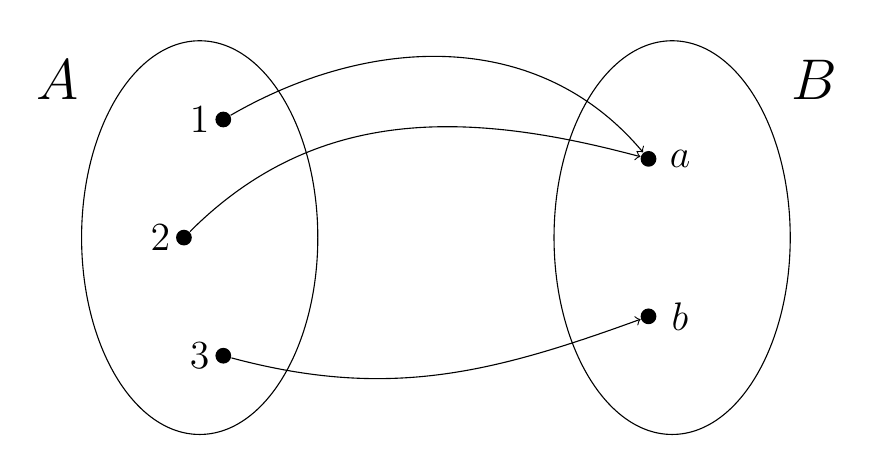
\begin{tikzpicture}
            \node[circle,fill,inner sep=0pt,minimum size=0.2cm] (A1) at (-2.7, 1.5) {};
            \node[circle,fill,inner sep=0pt,minimum size=0.2cm] (A2) at (-3.2, 0.0) {};
            \node[circle,fill,inner sep=0pt,minimum size=0.2cm] (A3) at (-2.7, -1.5) {};
            \node[circle,fill,inner sep=0pt,minimum size=0.2cm] (Ba) at (2.7, 1.0) {};
            \node[circle,fill,inner sep=0pt,minimum size=0.2cm] (Bb) at (2.7, -1.0) {};
 
            \draw (-3, 0) ellipse (1.5cm and 2.5cm);
            \node at (-4.8, 2) { \huge $A$ };

            \node at (-3.0, 1.5) { \Large $1$ };
            \node at (-3.5, 0.0) { \Large $2$ };
            \node at (-3.0, -1.5) { \Large $3$ };

            \draw (3, 0) ellipse (1.5cm and 2.5cm);
            \node at (4.8, 2) { \huge $B$ };

            \node at (3.1, -1.0) { \Large $b$ };
            \node at (3.1, 1.0) { \Large $a$ };

            \draw[->] (A1) to [out=30,in=130] (Ba);
            \draw[->] (A2) to [out=45,in=165] (Ba);
            \draw[->] (A3) to [out=-15,in=200] (Bb);

        \end{tikzpicture}
    \end{figure}

\end{frame}

\begin{frame}[fragile]{Exemplo de relação que não é função}

    \begin{figure}[h]
        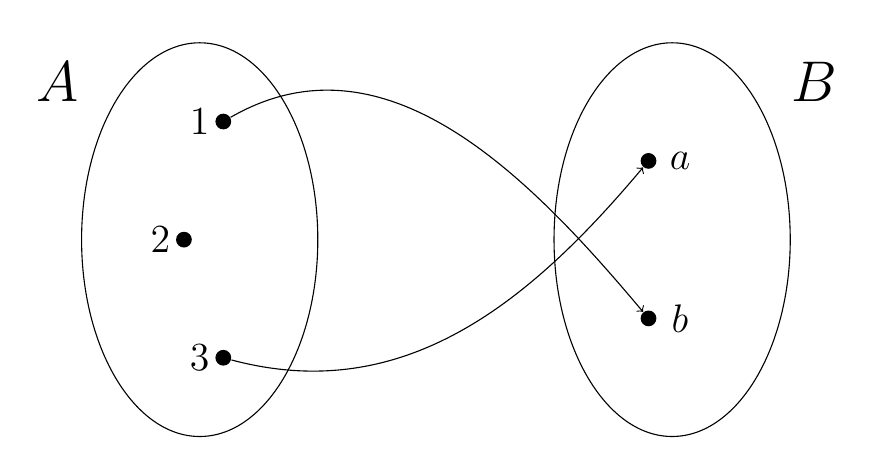
\begin{tikzpicture}
            \node[circle,fill,inner sep=0pt,minimum size=0.2cm] (A1) at (-2.7, 1.5) {};
            \node[circle,fill,inner sep=0pt,minimum size=0.2cm] (A2) at (-3.2, 0.0) {};
            \node[circle,fill,inner sep=0pt,minimum size=0.2cm] (A3) at (-2.7, -1.5) {};
            \node[circle,fill,inner sep=0pt,minimum size=0.2cm] (Ba) at (2.7, 1.0) {};
            \node[circle,fill,inner sep=0pt,minimum size=0.2cm] (Bb) at (2.7, -1.0) {};
 
            \draw (-3, 0) ellipse (1.5cm and 2.5cm);
            \node at (-4.8, 2) { \huge $A$ };

            \node at (-3.0, 1.5) { \Large $1$ };
            \node at (-3.5, 0.0) { \Large $2$ };
            \node at (-3.0, -1.5) { \Large $3$ };

            \draw (3, 0) ellipse (1.5cm and 2.5cm);
            \node at (4.8, 2) { \huge $B$ };

            \node at (3.1, -1.0) { \Large $b$ };
            \node at (3.1, 1.0) { \Large $a$ };

            \draw[->] (A1) to [out=30,in=130] (Bb);
            \draw[->] (A3) to [out=-15,in=230] (Ba);

        \end{tikzpicture}
    \end{figure}

\end{frame}


\begin{frame}[fragile]{Exemplo de relação que não é função}

    \begin{figure}[h]
        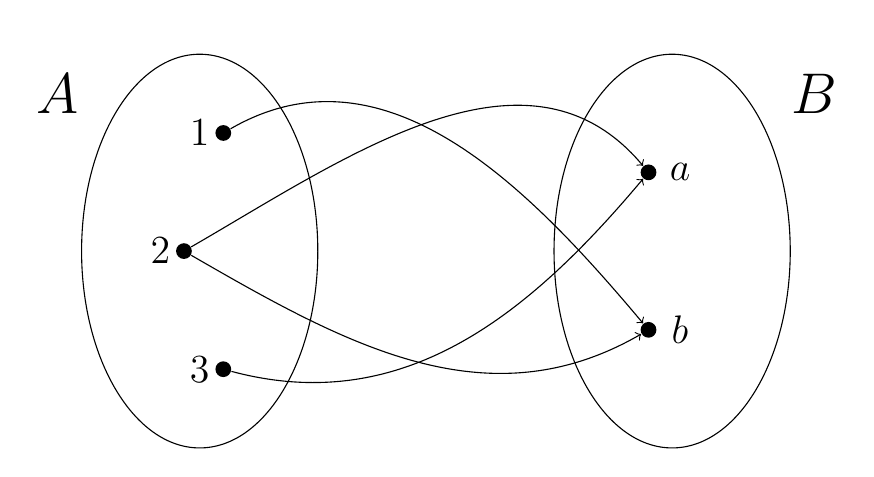
\begin{tikzpicture}
            \node[circle,fill,inner sep=0pt,minimum size=0.2cm] (A1) at (-2.7, 1.5) {};
            \node[circle,fill,inner sep=0pt,minimum size=0.2cm] (A2) at (-3.2, 0.0) {};
            \node[circle,fill,inner sep=0pt,minimum size=0.2cm] (A3) at (-2.7, -1.5) {};
            \node[circle,fill,inner sep=0pt,minimum size=0.2cm] (Ba) at (2.7, 1.0) {};
            \node[circle,fill,inner sep=0pt,minimum size=0.2cm] (Bb) at (2.7, -1.0) {};
 
            \draw (-3, 0) ellipse (1.5cm and 2.5cm);
            \node at (-4.8, 2) { \huge $A$ };

            \node at (-3.0, 1.5) { \Large $1$ };
            \node at (-3.5, 0.0) { \Large $2$ };
            \node at (-3.0, -1.5) { \Large $3$ };

            \draw (3, 0) ellipse (1.5cm and 2.5cm);
            \node at (4.8, 2) { \huge $B$ };

            \node at (3.1, -1.0) { \Large $b$ };
            \node at (3.1, 1.0) { \Large $a$ };

            \draw[->] (A1) to [out=30,in=130] (Bb);
            \draw[->] (A2) to [out=30,in=130] (Ba);
            \draw[->] (A2) to [out=-30,in=210] (Bb);
            \draw[->] (A3) to [out=-15,in=230] (Ba);

        \end{tikzpicture}
    \end{figure}

\end{frame}

\begin{frame}[fragile]{Funções notáveis}

    \begin{enumerate}
        \item A função \textbf{identidade} $\mathrm{id}: A\to A$, tal que $\mathrm{id}(x) = x$.

        \item A \textbf{adição} $a: B\times B \to B$, onde $a(x, y) = x + y$.
 
        \item A função \textbf{delta de Kronecker} $\delta: \mathbb{Z}\times \mathbb{Z}\to 
            \lbrace 0, 1\rbrace$, dada por
            \[
                \delta_{ij} = \left\lbrace \begin{array}{ll} 1, & \mbox{se}\ i = j, \\
                                                             0, & \mbox{caso contrário}\\
                                           \end{array} \right.
            \]

        \item A função de \textbf{decisão} $d_X: Y\to \lbrace \mathtt{True, False}\rbrace$, onde
            $d_X(y) = \mathtt{True}$ se $y\in X$; caso contrário, $d_X(y) = \mathtt{False}$.

        \item A função \textbf{logaritmo natural} $\ln: \mathbb{R^+}\to \mathbb{R}$, definida 
        abaixo
        \[
            \ln(x) = \int_1^x \frac{1}{t} dt
        \]

    \end{enumerate}

\end{frame}

\begin{frame}[fragile]{Domínio, imagem e gráfico}

    \begin{block}{Domínio e imagem de uma função $f$ de $A$ em $B$}
        Seja $f$ uma função de $A$ em $B$. O conjunto $A$ é denominado \textbf{domínio} da
            função $f$, e o conjunto $B$ o \textbf{contradomínio} de $f$. Além disso, o conjunto
        \[
            Img(f) = \lbrace b \in B\ |\ \exists\, a\in A\ \mbox{tal que}\ f(a) = b \rbrace
        \]
        é a \textbf{imagem} da função $f$. Outra notação comum para o conjunto imagem de $f$ é 
        $f(A)$.
    \end{block}

    \vspace{0.05in}

    \begin{block}{Gráfico de uma função}
        Seja $f$ uma função de $A$ em $B$. O gráfico de $f$ é o conjunto
        \[
            Gr(f) = \lbrace (x, f(x))\ |\ x\in A\rbrace
        \]
    \end{block}

\end{frame}

\begin{frame}[fragile]{Composição de funções}

    \begin{block}{Função composta}
        Sejam $f: A\to B$ e $g: C\to D$ duas funções. Se $f(B)\subset C$, então a função
            composta $h: A\to D$ é definida como
        \[
            h(x) = (g\circ f)(x) = g(f(x))
        \]
    \end{block}

    \vspace{0.2in}

    \textbf{Observação}: Em geral, $(g\circ f)(x) \neq (f\circ g)(x)$ (pode ser que $(f\circ g)(x)$
        nem esteja, de fato, definida).

\end{frame}
